%{ 
% This opens a block comment for MATLAB and Octave
\documentclass[12pt]{article}

\usepackage{mathptmx}
\usepackage{setspace}
\usepackage[margin=1.0in]{geometry}
\usepackage{authblk}
\usepackage{abstract}
\usepackage{amsmath}
\usepackage[usenames,dvipsnames,svgnames,table]{xcolor}


% \usepackage{caption}
% \captionsetup{labelsep=none,textformat=empty}

\usepackage{subcaption}

% \usepackage[nomarkers]{endfloat}

% % change the way captions are displayed beneath figures (Only display figure number)
% \renewcommand{\@makecaption}[2]{{\centering   \vskip\abovecaptionskip \bfseries #1} #2}
% \renewcommand{\@makecaptionZ}[2]{%
%   \vskip\abovecaptionskip
%   \sbox\@tempboxa{#1}%
%   \ifdim \wd\@tempboxa >\hsize
%     #1\par
%     \else
%     \global \@minipagefalse
%   \hb@xt@\hsize{\hfil\box\@tempboxa\hfil}%
%   \fi
%   \vskip\belowcaptionskip}

% % Change the way Figure and Table captions appear in List of Figures/Tables
% \renewcommand{\l@figure}[2]{%
%  \setlength\@tempdima{2.3em}%
%  \noindent\hspace*{1.5em}Figure #1\hfil\newline }
% \renewcommand{\l@table}[2]{%
%  \setlength\@tempdima{2.3em}%
% \noindent\hspace*{1.5em}Table #1\hfil\newline }

\usepackage{graphicx}
\usepackage{booktabs}
\usepackage{cleveref}

\usepackage{verbatim}
\usepackage{anyfontsize}
\usepackage{nameref}
\usepackage{nicefrac}
\usepackage{float}
\usepackage{bm}
\usepackage{multirow}
\usepackage[ruled,vlined,linesnumbered]{algorithm2e}
\usepackage{tikz}
\usepackage[group-separator={,}]{siunitx}
\usepackage{xspace}

\usepackage{verbatim}
\usepackage{csvsimple}
\usepackage{listings}
\usepackage{color} %red, green, blue, yellow, cyan, magenta, black, white
\definecolor{mygreen}{RGB}{28,172,0} % color values Red, Green, Blue
\definecolor{mylilas}{RGB}{170,55,241}
\definecolor{backcolour}{rgb}{0.95,0.95,0.92}


\newenvironment{matlab}{\comment}{\endcomment}    
\newenvironment{octave}{\comment}{\endcomment}    
\newenvironment{matlabv}{\verbatim}{\endverbatim} 
\newenvironment{octavev}{\verbatim}{\endverbatim}

\usepackage{hyperref}
\usepackage[numbers]{natbib}
\bibliographystyle{natbib}

% after hypperref, do this to remove figure captions properly
% \def\onlylabel \label#1#2\par{\label{#1}}
% \let\origcaption=\@caption
% \long\def\@caption#1[#2]#3{\origcaption#1[#2]{\onlylabel #3}}

\doublespacing
\renewcommand{\abstractname}{}    % clear the title
\renewcommand{\absnamepos}{empty} % originally center

\newcommand{\note}[1]{\textcolor{orange}{note: #1}}
\newcommand{\forexample}{e.g.\@\xspace}
\newcommand{\thatis}{i.e.\@\xspace}
\newcommand{\viz}{viz.\@\xspace}
\newcommand{\andothers}{et al.\@\xspace}
\newcommand{\totCount}[1]{\ensuremath{T(#1)}}
\newcommand{\tset}{\ensuremath{\mathcal{T}}\xspace}
\newcommand{\rset}{\ensuremath{\mathcal{R}}\xspace}
\newcommand{\kmersof}[1]{\ensuremath{\textrm{\texttt{kmers}}(#1)}\xspace}
\newcommand{\card}[1]{\ensuremath{\left|#1\right|}\xspace}
\newcommand{\func}[3]{\ensuremath{#1 : #2 \to #3}\xspace}
\newcommand{\sfindex}[2]{\ensuremath{I_{#1}({#2})}\xspace}
\newcommand{\eqClass}[1]{\ensuremath{\left[#1\right]}\xspace}
\newcommand{\arrElem}[2]{\ensuremath{#1\left(#2\right)}\xspace}
\renewcommand{\vec}[1]{\ensuremath{\mathbf{#1}}}
\newcommand{\norm}[1]{\ensuremath{\left|\left|#1\right|\right|}}
\newcommand{\kmer}{k-mer\xspace}
\newcommand{\kmers}{k-mers\xspace}
\renewcommand{\bowtie}{Bowtie\xspace}
\newcommand{\rsem}{RSEM\xspace}
\newcommand{\express}{eXpress\xspace}
\newcommand{\cufflinks}{Cufflinks\xspace}
\newcommand{\tophat}{TopHat\xspace}
\newcommand{\sailfish}{Sailfish\xspace}
\newcommand{\suppfigref}[1]{Supplementary Fig.~\ref{#1}\xspace}
\newcommand{\suppref}[1]{Supplementary Material, Sec.~\ref{#1}\xspace}
\newcommand{\suppnoteref}[1]{Supplementary Material, Sec.~\ref{#1}\xspace}
\newcommand{\methodseqnref}[1]{Methods, Eqn.~\ref{#1}\xspace}
\newcommand{\methodsalgref}[1]{Methods, Alg.~\ref{#1}\xspace}
\newcounter{countSupNote}
%\setcounter{page}{0}
\def\tm{\leavevmode\hbox{$\rm {}^{TM}$}}

\title{Linear Algebraic and Boolean Analysis of Genomic Topology}

\author[1]{Shengyun Peng}
\author[1]{Cai Huang}
\author[1]{Peter Audano}
\author[1]{Fredrik O. Vannberg}
\affil[1]{Parker H. Petit Institute for Bioengineering and Biosciences, School of Biology, Georgia Institute of Technology, Atlanta, Georgia 30332, USA}

\date{}

\begin{document}
\maketitle

\begin{abstract}   
ABSTRACT 
\end{abstract}
To date the comparison of genomic DNA sequences\cite{Pruitt:2005aa} have routinely utilized shorter conserved regions for comparative genomics. Current phylogenetic analysis therefore can create divergent results based on which genetic loci are utilized for this analysis\cite{Salichos:2013aa}. Sequence similarity is also commonly determined by first carrying out gap penalty pairwise alignments\cite{Altschul:1990aa}\cite{Vingron:1994aa}\cite{Morgenstern:1996aa} for a set of sequences, and the similarity is quantified based upon this alignment. This approach, however, has limitations and is primarily utilized to compare relatively conserved sequences and is also dependent upon the algorithm utilized to create the alignment.  From first principles we here develop a framework for encoding nucleic acid sequences into fixed length sections (k-mers)\cite{Chor:2009aa}\cite{Grabherr:2011aa} which we utilize to create an invariant pairwise distance of total information content of over $\sim4,000$ bacteria\cite{Doolittle:2002aa} and viruses, revealing important cryptic relationships not previously reported. To date k-mer strategies have been utilized by nearly all short read DNA alignment strategies, including de Bruijn-type\cite{Compeau:2011aa} combinatorial mathematics and Burrows-Wheeler transform\cite{Adjeroh:2002aa} (BWT) algorithm to efficiently align sequences. Our framework adds another layer of abstraction to this field by creating an invariant encoding heuristic for k-mers that allows for the efficient analysis and computation of genome similarities. This invariant encoding framework is computable by linear algebra and also diverse Boolean, logic and bit operations of discrete mathematics. In addition to orthogonal transformation of this dataset we also show pairwise differential occupancy (which we term $\Delta {\Gamma _k}$) of these data structures for hierarchical clustering of genomic sequence. To our knowledge we define the first global clustering of entire bacterial and viral genomes, which we define here as genomic topology, which led to the discovery of a number of novel cryptic genomic associations between specific viral phages\cite{Sampson:2009aa} and bacteria. This formalization of genomic relationships yields an invariant pairwise differential occupancy ($\Delta {\Gamma _k}$) metric between all species based upon global information content of each genome, irrespective of Kingdom, and finally allows a universal complete encoding for species that was lacking in previous approaches. \\ 
The exponential growth in sequencing information of organisms of all Kingdoms has greatly increased our understanding of the diversity of genomes and genomic complexity. In order to help formalize and explore genomic encoding we have created a sparse k-mer encoding system wherein genomic data is stored in an identical format that allows for global computations across all genomic data, regardless of homology. To date there has been a distinct lack of fundamental organization of genomic data, with primarily ad hoc analysis of genome similarity using subsets of evolutionarily conserved genes.\\
We created a universal encoding system to store k-mer data in sparse linear vector form as well as an equivalent $n \times $n square sparse matrix form (Supporting Online Material Fig. 1). Briefly, our system utilizes a sparse vector that contains ${4^k}$ elements, arrayed in ascending order by the binary representation of the k-mer, where $\left\{ {A = 00,{\rm{ }}C = 01,{\rm{ }}G = 10,{\rm{ }}T = 11} \right\}$. For these sparse vectors we define tau $({\Gamma _k})$ by the number of non-zero elements divided by ${4^k}$ elements , where k represents the k-mer length. We routinely also transform this binary k-mer representation into a decimal number as seen in Fig.~\ref{fig:encoding}A.In order to optimize this k-mer analysis we authored KAnalyze~\cite{Audano:2014aa}, which is a fast and extensible \kmer suite with APIs specific for this process.\\
From these first principles, we sought ways to globally analyze these sparse linear vectors. Using standard linear algebra approaches it is possible to complete orthogonal transformations of this data (Fig.~\ref{fig:encoding}B). In one manifestation we carry out hierarchical principle component analysis (hPCA)~\cite{Peterson:2002aa} (see Methods) of the combined genomic sparse vectors of multiple species, allowing for distance calculations in n-dimensional space, with the closest shared information content giving the smallest distance using three (or more) components. These first three components can then be used to create a three dimensional plot of the distances between the sparse vectors for each genome sequence (Fig.~\ref{fig:encoding}B). In a similar manner, it is possible to carry out global Boolean analysis on these sparse vectors in a pairwise fashion. By arraying the sparse vectors in an invariant format, with full encoding, it is trivial to carry out pairwise discrete functions for any logic gate functions including {AND, OR, XOR} as seen in Figure 1B. One simple metric is the resultant value of the XOR Boolean operator between two sparse vectors, which we here define as delta tau ($\Delta {\Gamma _k}$), or differential occupancy, where k defines the k-mer length (see Methods).


\begin{figure}
%
\begin{center}
%
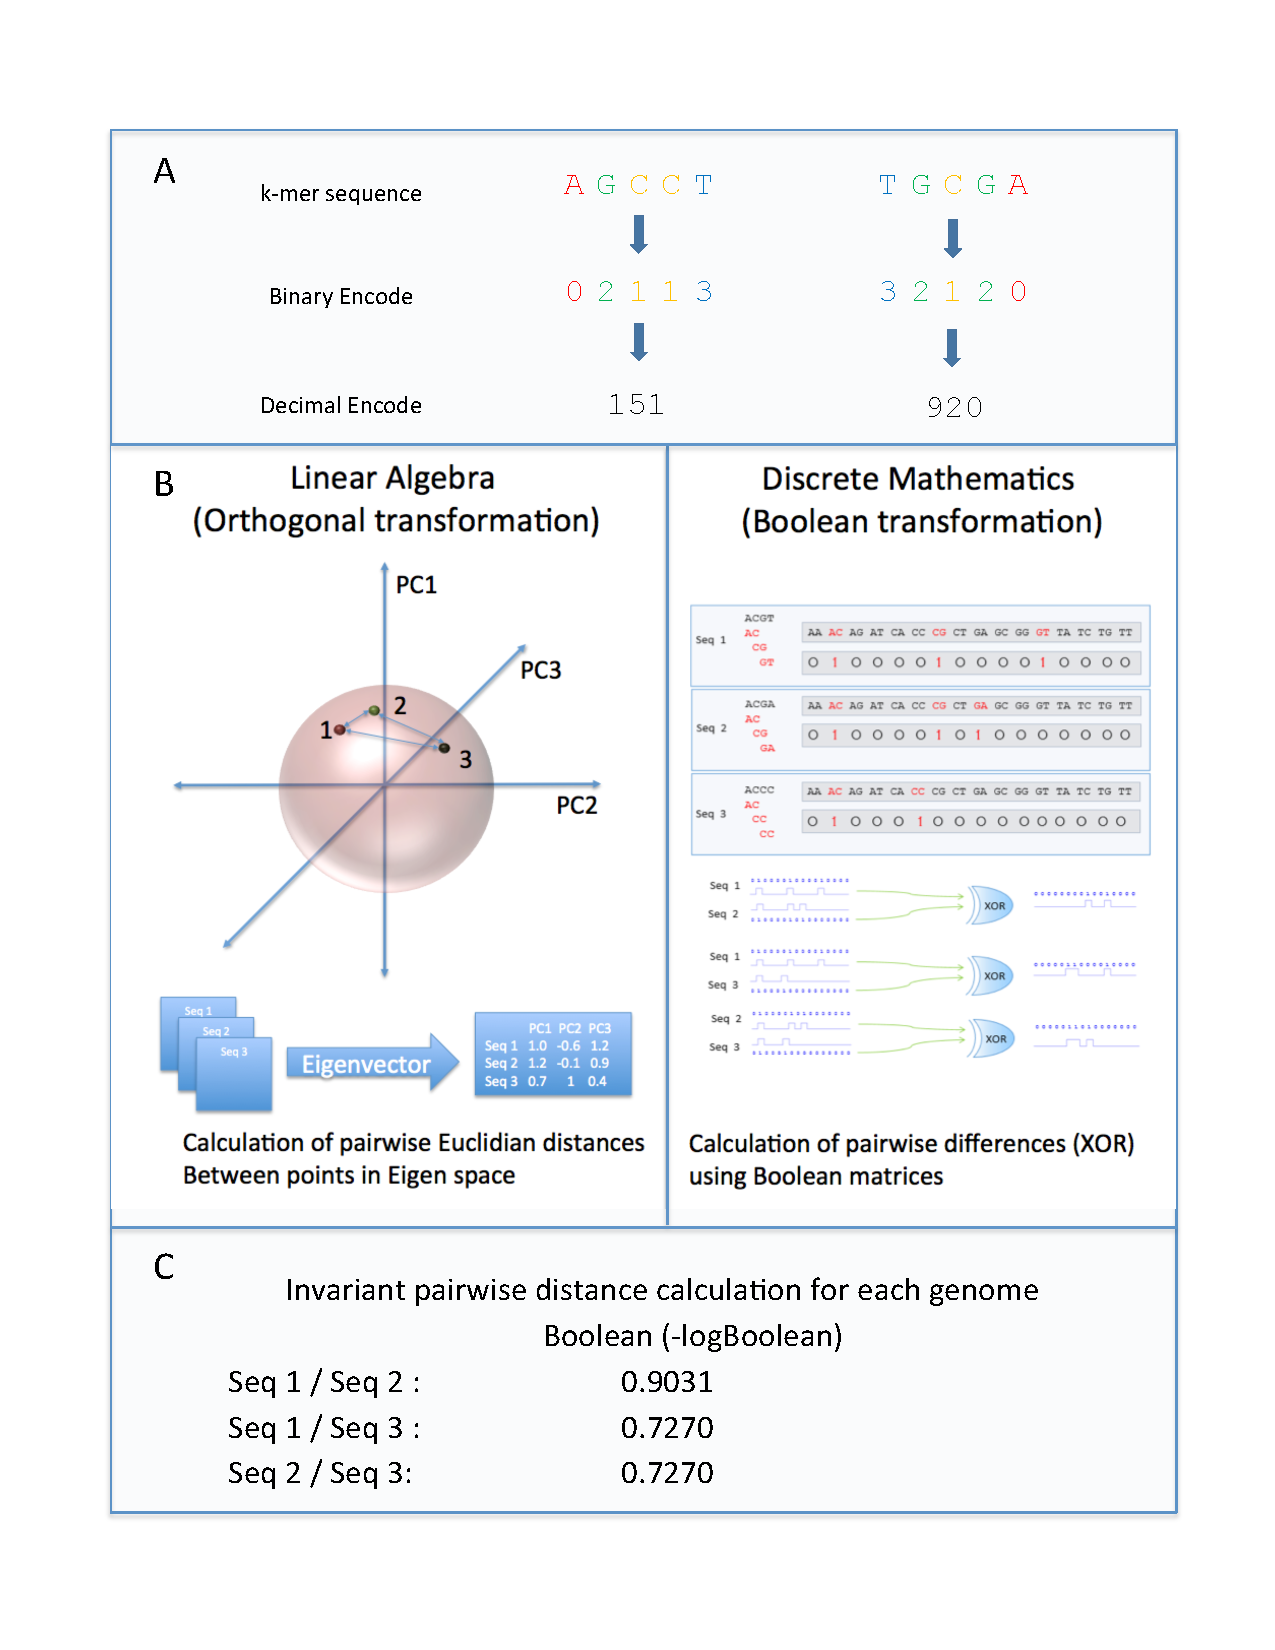
\includegraphics[width=0.7\textwidth]{Universal_K-mer_encoding_and_computation.pdf}
%
\caption{\label{fig:encoding}Universal K-mer encoding and computation.  A) Universal encoding defined using the Quaternary-Decimal encoding system. B) Linear algebra forms analyzes a variety of orthogonal transformation / eigenvector calculations. Discrete mathematics enables Boolean analysis using the full complement discrete functions including AND, OR, and XOR.}
%
\end{center}
\end{figure}

We start by carrying out the hPCA analysis of 578 bacterial genomes in the NCBI bacterial database.  And we plot log transformed pairwise distance of these bacterial genomes base on hPCA. By z-transforming the pairwise $ - \log (\Delta {\Gamma _k})$ data we see a desirable and expected association between species-based similarities between k-mer encoding, and define $z >  = 2$ as closely related species. We formalize this association and speculate that this relationship follows a power law association (Fig.~\ref{fig:distance}A), which appear to be inherent in natural genomic topologies of biological systems. We here show punctuate peaks (Fig.~\ref{fig:distance}B) of closely related species within a sea of random or near random associations. Similarly, in calculating genomic topologies of all pairwise $ - \log (\Delta {\Gamma _k})$ species (Fig.~\ref{fig:distance}C, D) will be defined as those that reside within the k-mer topology within the exponential function of arrayed pairwise relationships, indicating a ``null'' and ``positive''space. For these closely related species we see ${R^2}$ value of 0.87 between the hPCA and Boolean analysis (Fig.~\ref{fig:distance}E), for the species with a pairwise relationship of $z>=2$. We show the density plot of all pairwise comparisons (extended Fig. 1, Supporting Online Material Table 1). Using this $\Delta {\Gamma _k}$ we apply hierarchical clustering and obtain expected clustering of these bacterial genomes (Fig.~\ref{fig:clustering}). 


\begin{figure}
%
\begin{center}
%
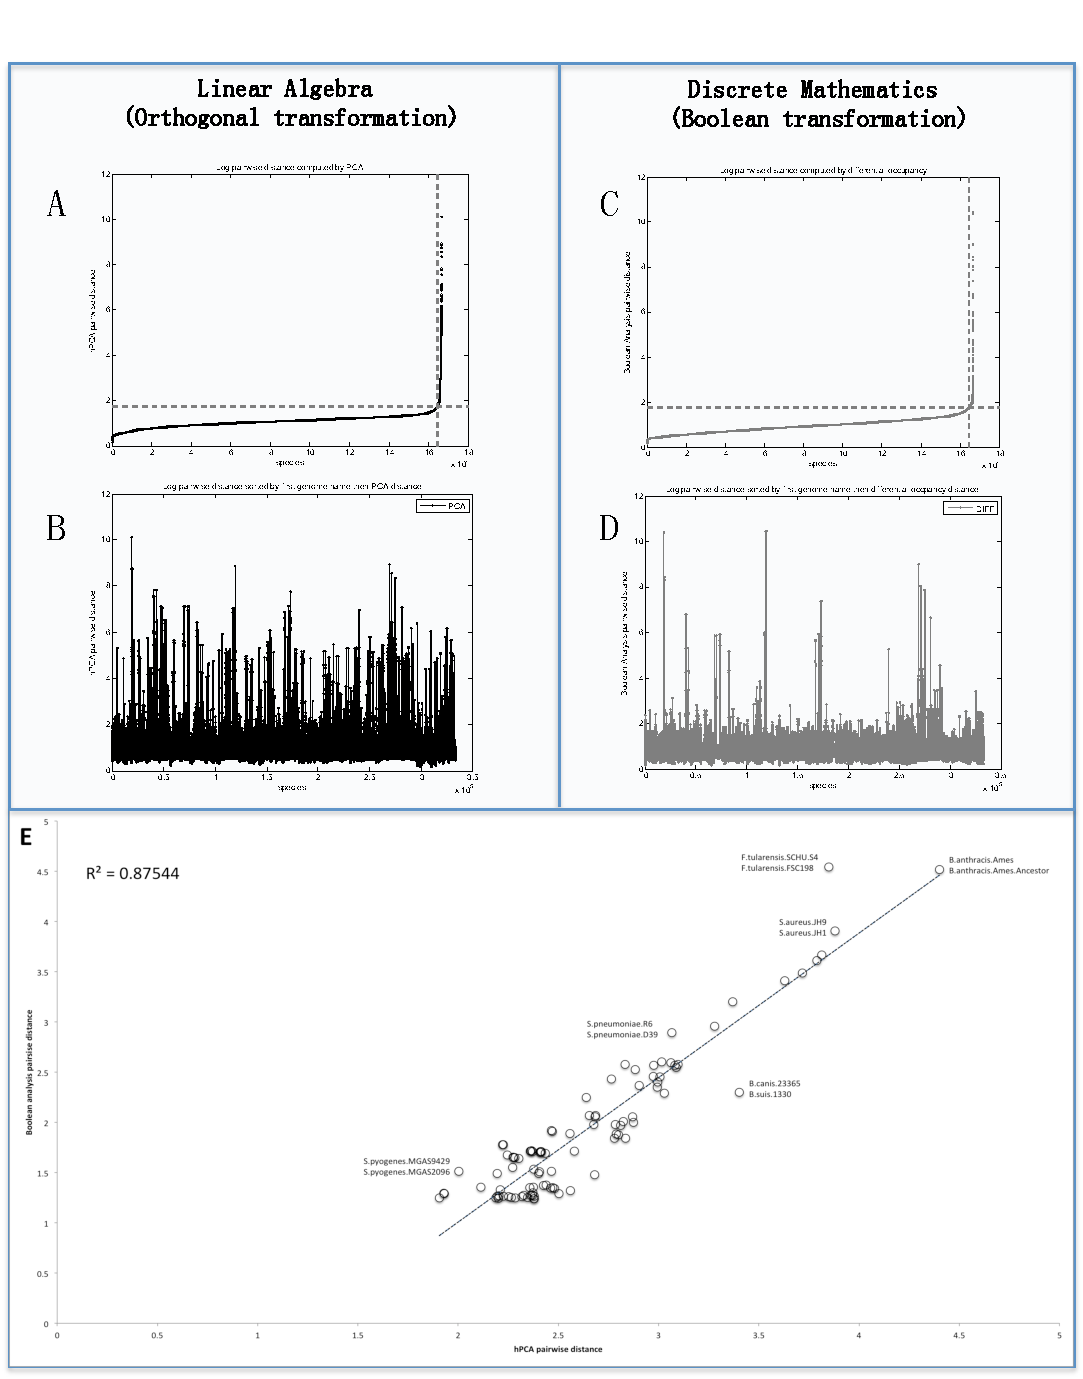
\includegraphics[width=0.7\textwidth]{Pairwise_distance.pdf}
%
\caption{\label{fig:distance}Pairwise distance.  A) Sorted Log pairwise distance computed by hPCA; B) Unsorted Log pairwise distance computed by hPCA; C) Sorted Log pairwise distance computed by Boolean Analysis; D) Unsorted Log pairwise distance computed by Boolean Analysis; E) Pairwise distance from hPCA and Boolean analysis relationship. }
%
\end{center}
\end{figure}


\begin{figure}
%
\begin{center}
%
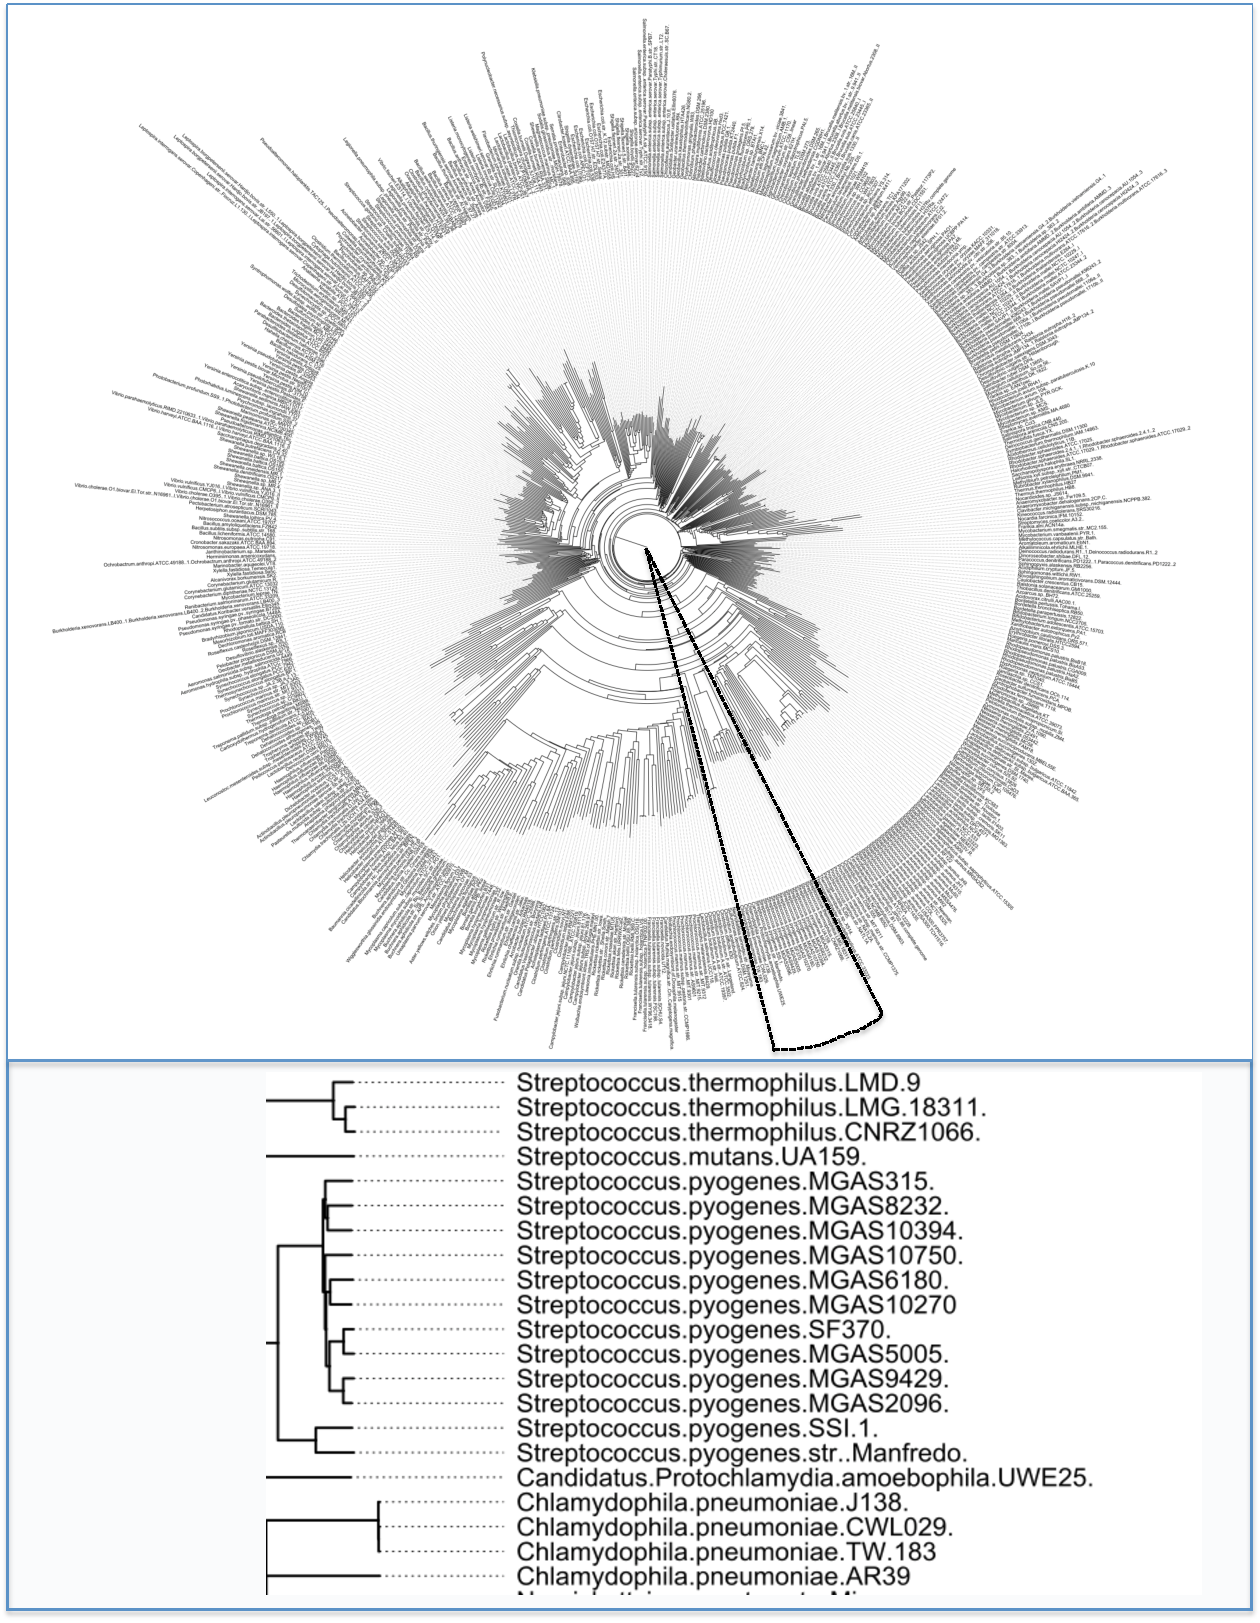
\includegraphics[width=0.7\textwidth]{Hierarchical_clustering.pdf}
%
\caption{\label{fig:clustering}Hierarchical clustering. Zoom in part of the hierarchical clustering generated by differential occupancy \(complete tree in Supporting Online Material, 578_10mer_diff_tree\).}
%
\end{center}
\end{figure}

This technique enables the comparison of highly divergent genomic sequences and we utilize these heuristics to perform hPCA clustering of bacterial and viral sequences (extended Fig. 2). In addition to finding a number of known relationships between bacteria and viruses, we also found evidence of previously cryptic relationships between these bacterial and viral genomes. From linear algebra genomic topology analysis we find examples that make sense in terms of likely horizontal gene transfer such as a close link between \emph{Sulfolobus virus STSV1} and \emph{Sulfolobus islandicus M}; \emph{Sulfolobus virus STSV1} and \emph{Sulfolobus solfataricus}; \emph{Sulfolobus virus STSV1} and \emph{Sulfolobus acidocaldarius}; \emph{Sulfolobus virus STSV1} and \emph{Sulfolobus tokodaii}~\cite{Xiang:2005aa}; \emph{Salmonella phage ST64B} and \emph{Escherichia coli ED1a}; \emph{Klebsiella phage phiKO2} and \emph{Escherichia coli O26}. However, this analysis also revealed several unexpected relationships between \emph{Klebsiella phage phiKO2} and \emph{Enterobacter cloacae EcWSU1}; \emph{Enterobacteria phage N15} and \emph{Pectobacterium atrosepticum SCRI1043}, among others. These relationships highly suggestive of shared genomic content through horizontal gene transfer, and provide a new perspective to examine these putative new relationships between of bacteria and viruses. We prepared a K-ermized data set of 2569 bacteria and 1754 virus sequences and hPCA (Supporting Online Material) analysis result for further study. \\
We demonstrate that our approach can analyze an ancient genome such as \emph{Acidianus bottle shaped virus}, which infect archaea~\cite{Haring:2005aa}, in the context of other viruses. By using grep function, we output pairwise relationship between Acidianus bottle shaped virus and all other species in our database, then we sorted by the hPCA distance. We find out close virus spices have stronger relationship than other random picked and bacteria (Fig.~\ref{fig:circus}). Also, we can to study the relationship between this virus and other bacteria. So we show a circus plot of several bacteria, which have low hPCA distance with the virus, and five random picked \emph{Methylobacterium} family bacteria (extended Fig. 3). We can see the \emph{Methylobacterium} family are far away from our virus, because they are less related than the \emph{Vulcanisaeta moutnovskia}~\cite{Gumerov:2011aa} to the virus, and it is an Archaea, which might be infected by \emph{Acidianus bottle shaped virus}. Besides, \emph{Caldivirga maquilingensis, Ignisphaera aggregans, Vulcanisaeta distribute, Desulfurococcus fermentans,} are all Archaea. This suggests that there is relationship between virus and infected bacteria on genome perspective. For another example, we can study on an unclassified sequence, and suggest classification. We pick an unclassified virus, \emph{Pyrococcus abyssi virus 1}. By using \emph{grep} function, we output relationship between this virus and all other species in our database. After sorting the output by hPCA distance, we study the top 12 species (log-transformed hPCA distance higher than 2.5) and their lineage (extended table 1). From the table, we can see that most of these known species are belong to \emph{Viruses; dsDNA viruses, no RNA stage; Caudovirales} family. So we can positively suggest that Pyrococcus abyssi virus 1 can be classified to \emph{Viruses; dsDNA viruses, no RNA stage; Caudovirales}. \\
In the past it was not possible to adequately compare complete genomic content between two species due to the inability to align dissimilar sequence. Therefore although claims of genomic topology creating certain maxima and trough minima, this was not possible to properly test. Using our analysis, it does indeed appear that there is a specific power law effect that describes the overall genomic topology between species, with a sharp exponential decay in genomic topology between two different species. This, again, has been suggested but we feel that our result is one of the clearest attempts to show such a genomic topology. \\
We demonstrate the ability to cluster within species from first principles using genomic topology calculations without additional levels of abstraction. We show that optimized discrete calculations on global k-mer space qualitatively work as well as traditional linear algebra-based orthogonal transformations eigen value-based principle component analysis. Although laboratories can and will use analysis of higher levels of abstraction such as the case of PCA and multiple dimensional scaling, it is our opinion that it is easier to intuit intellectually discrete calculations of these higher order matrices verses taking into account the eigen vector space. An important distinction, which is always troubling with PCA and MDS type of analysis is that the origin of the variation is lost in the calculation, with the inability to determine the origin of the variation. Discrete systems do not face such restrictions, and our system creates the ability to real time cluster and reveals the origin of the variation at the same time, creating a use case that is relevant to pharmacological development. Optimizing our k-mer size to allow for the global creation of siRNA sequences against a known and novel virus we demonstrate that our k-mer system does well to not only process this but also be able to compare sequences in real time with approach we present. The simplicity of this system, along with the considerable advancements that can be made to further innovate from this adds a great deal we believe to the toolkit of mathematics for biologists and we hope that brings into sharper focus quantitative biology principles moving ahead. It is not lost on us that a similar encoding system using \kmer can also be carried out for amino acid sequences encoded within organisms, and the parity between such genomic and proteomic data will also be useful in comparative analysis of species. Indeed philosophically this brings to the fore arguments for such numerical taxonomy approaches whereby additional data streams can be added into such analysis, allowing for quantitative assessments of species, including morphological, developmental and even neuronal encoding. These to date can be seen as ad hoc, but formalization approaches abound, such as the National Institutes of Health Brain Mapping Initiative, which can allow for formalization of such systems. We present some preliminary analysis of this, but further more sophisticated analysis of genome, proteomic and other feature space is possible using a similar model of creating invariant data structures that allow for like for like comparisons of data sets. It should be noted that this is not closed to inter-species analysis, indeed use cases abound that make intra-species analysis informative. Examples include analysis of virulent E. coli strains, or viral outbreaks scenarios. Our laboratory is working closely with multiple Centers for Disease Control branches to implement such analysis to allow for near complete automation of such pairwise $\Delta {\Gamma _k}$ analytics during outbreak scenarios. \\ 


\begin{figure}
%
\begin{center}
%
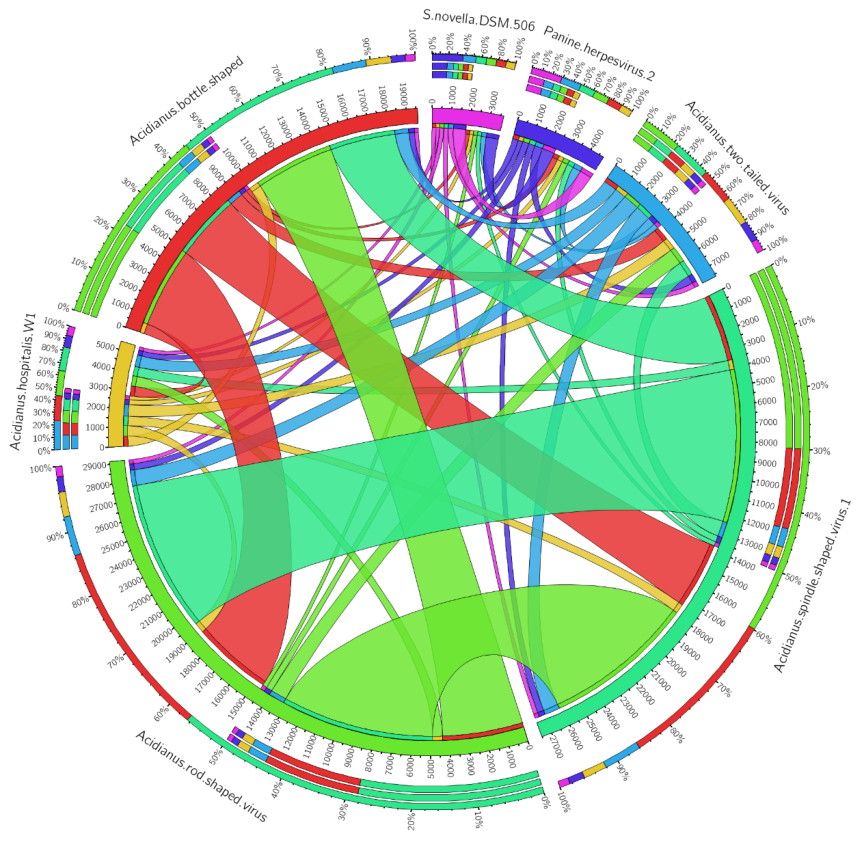
\includegraphics[width=0.7\textwidth]{Circus_plot_of_five_Acidianus_family_virus.pdf}
%
\caption{\label{fig:circus}Circus plot of five Acidianus family virus, one random herpesvirus and one random Starkeya.novella bacteria. The pairwise relationship (extended table 3) are present by 10/(hPCA distance), so the thicker the connect line is, the closer they are.}
%
\end{center}
\end{figure}



\section*{Methods}
\label{sec:methods}

We provide a small data set to demonstrate the method we used to calculate the pairwise distance. The test data set is random picked 4 kmerized virus files with k length equal to 8, and stored as \emph{csv} file. Each column is a sparse vector and represents one virus. sequence.

\paragraph{hPCA} 

The hPCA analysis is base on PCA. So we perform a PCA calculation among the normalized dataset and use only the main components to calculate the distance between viruses. Here we provide a R function to calculate the hPCA distance on kmerized data set. For normalization we  subtract each column of data by its mean and divided by its stand deviation, and the distance funtion we uesd is \emph{euclidean} distance. 

 

\paragraph{Boolean Analysis} We define the term differential occupancy as the XOR function between two sparse vectors that derives resultant sparse vector followed by summing the number of non-zero elements then dividing by $4^k$. The more similar two genomes the smaller the number of resultant non-zero elements after the XOR calculation, resulting in a number that approaches zero for the same species. Herer is the matlab code for iterate the test data set and calculate the differential occupancy.


\noindent The pairwise distance reault shows in Table \ref{table:two}.Each number represents the pairwise diffrential occupancy of two virus, and the smaller the number is, the closer they are.


\newpage 
%\bibliographystyle{abbrv}
\bibliography{Genomic_Topology_2014}

%\processdelayedfloats

\newpage

%===========================================================================================
%\begin{center}
%{\large \singlespacing \sailfish: Alignment-free Isoform Quantification from RNA-seq Reads using Lightweight Algorithms\\}
%Rob Patro, Stephen M.Mount and Carl Kingsford
%\end{center}

%\captionsetup{labelfont=bf}
%\setcounter{figure}{0}
%\setcounter{page}{1}
%\renewcommand{\figurename}{Supplementary Figure}
%\section{Supplementary Material}
%\label{sec:supinf}


\end{document}
